\documentclass[letterpaper]{article}
\usepackage[margin=1in]{geometry}
\usepackage[utf8]{inputenc}
\usepackage{textcomp}
\usepackage{amssymb}
\usepackage{natbib}
\usepackage{graphicx}
\usepackage{gensymb}
\usepackage{amsthm, amsmath, mathtools}
\usepackage[dvipsnames]{xcolor}
\usepackage{enumerate}
\usepackage{mdframed}
\usepackage[most]{tcolorbox}
\usepackage{csquotes}
% https://tex.stackexchange.com/questions/13506/how-to-continue-the-framed-text-box-on-multiple-pages

\tcbuselibrary{theorems}

\newcommand{\R}{\mathbb{R}}
\newcommand{\Z}{\mathbb{Z}}
\newcommand{\N}{\mathbb{N}}
\newcommand{\Q}{\mathbb{Q}}
\newcommand{\C}{\mathbb{C}}
\newcommand{\code}[1]{\texttt{#1}}
\newcommand{\mdiamond}{$\diamondsuit$}
\newcommand{\PowerSet}{\mathcal{P}}
\newcommand{\Mod}[1]{\ (\mathrm{mod}\ #1)}
\DeclareMathOperator{\lcm}{lcm}

%\newtheorem*{theorem}{Theorem}
%\newtheorem*{definition}{Definition}
%\newtheorem*{corollary}{Corollary}
%\newtheorem*{lemma}{Lemma}
\newtheorem*{proposition}{Proposition}


\newtcbtheorem[number within=section]{theorem}{Theorem}
{colback=green!5,colframe=green!35!black,fonttitle=\bfseries}{th}

\newtcbtheorem[number within=section]{definition}{Definition}
{colback=blue!5,colframe=blue!35!black,fonttitle=\bfseries}{def}

\newtcbtheorem[number within=section]{corollary}{Corollary}
{colback=yellow!5,colframe=yellow!35!black,fonttitle=\bfseries}{cor}

\newtcbtheorem[number within=section]{lemma}{Lemma}
{colback=red!5,colframe=red!35!black,fonttitle=\bfseries}{lem}

\newtcbtheorem[number within=section]{example}{Example}
{colback=white!5,colframe=white!35!black,fonttitle=\bfseries}{def}

\newtcbtheorem[number within=section]{note}{Important Note}{
        enhanced,
        sharp corners,
        attach boxed title to top left={
            xshift=-1mm,
            yshift=-5mm,
            yshifttext=-1mm
        },
        top=1.5em,
        colback=white,
        colframe=black,
        fonttitle=\bfseries,
        boxed title style={
            sharp corners,
            size=small,
            colback=red!75!black,
            colframe=red!75!black,
        } 
    }{impnote}
\usepackage[utf8]{inputenc}
\usepackage[english]{babel}
\usepackage{fancyhdr}
\usepackage[hidelinks]{hyperref}

\pagestyle{fancy}
\fancyhf{}
\rhead{CSE 105}
\chead{Wednesday, February 09, 2022}
\lhead{Lecture 10}
\rfoot{\thepage}

\setlength{\parindent}{0pt}

\begin{document}

\section{Pushdown Automata (2.2)}
We now introduce a new type of computational model called the \textbf{pushdown automata}, which is essentially like a nondeterministic finite automata but with an extra component called a \textbf{stack}. The stack provides additional memory beyond the finite amount available in the control, additionally allowing us to recognize some nonregular languages. 

\bigskip 

Note that pushdown automata are \underline{equivalent in power} to context-free grammars, giving us the ability to decide which of the two we want to use to prove that a language is context-free. 


\subsection{The Idea}
The idea is that, at each step: 
\begin{enumerate}
    \item \textbf{Transition} to a new state based on the current state, letter read, \emph{and} the top letter of the stack. 
    \item Possibly push (or pop) a letter to (or from) the top of the stack. 
\end{enumerate}
We \emph{accept} a string if there is \textbf{some} sequence of states and \textbf{some} sequence of stack contents which processes the entire input string and ends in an accepting state. We assume that the stack is empty at the beginning, and don't necessarily care if the stack is empty at the end.

\subsection{Formal Definition}
As implied, the formal definition of a pushdown automaton is similar to that of a finite automaton, except for the stack. The stack is a device containing symbols drawn from some alphabet, and the machine may use different alphabets for its input and its stack. Therefore, we need to specify both an input alphabet $\Sigma$ and a stack alphabet $\Gamma$. 

\bigskip 

Recall that $\Sigma_{\epsilon} = \Sigma \cup \{\epsilon\}$; the same idea applies with $\Gamma_{\epsilon}$. Now, the domain of $\delta$ is $Q \times \Sigma_{\epsilon} \times \Gamma_{\epsilon}$. The idea behind this domain is that, given the current state $q \in Q$, next input symbol read $\sigma \in \Sigma_{\epsilon}$, and top symbol of the stack $\gamma \in \Gamma_{\epsilon}$, the machine can decide the next move. As usual, if $\sigma = \epsilon$, then the machine won't read a symbol from the input. Likewise, if $\gamma = \epsilon$, then the machine won't read a symbol from the stack.  

\bigskip 

We now consider the range of the $\delta$ function. It's possible that it can enter a new state and possibly write a symbol on top of the stack. This is indicated by some member of $Q \times \Gamma_{\epsilon}$. 

\begin{definition}{}{}
    A \textbf{pushdown automaton} is a 6-tuple $(Q, \Sigma, \Gamma, \delta, q_0, F)$, where $Q$, $\Sigma$, $\Gamma$, and $F$ are all finite sets, and
    \begin{enumerate}
        \item $Q$ is the set of states. 
        \item $\Sigma$ is the input alphabet. 
        \item $\Gamma$ is the stack alphabet.
        \item $\delta: Q \times \Sigma_{\epsilon} \times \Gamma_{\epsilon} \mapsto \PowerSet(Q \times \Gamma_{\epsilon})$ is the transition function.
        \item $q_0 \in Q$ is the start state. 
        \item $F \subseteq Q$ is the set of accept states. 
    \end{enumerate} 
\end{definition}
\textbf{Remark:} We write $a, b \mapsto c$ to signify that, when the machine is reading an $a$ from the input, it may replace the symbol $b$ on the top of the stack with a $c$; in other words, pop $b$ and push $c$. 
\begin{itemize}
    \item If $a = \epsilon$, then the machine may make this transition without reading any symbol from the input. 
    \item If $b = \epsilon$, then the machine may make this transition without readng any symbols from the stack, but it will push $c$ onto the stack. 
    \item If $c = \epsilon$, then the machine will pop $b$ from the stack but not push anything to the stack. 
\end{itemize}
\textbf{Note:} The formal definition of a PDA contains no explicit mechanism to allow the PDA to test for an empty stack. So, one trick that we can do is to initially push a special symbol \code{\$} on the stack. Then, if it ever sees the \code{\$} again, then it knows that the stack is effectively empty. 

\subsection{Computation of a Pushdown Automaton}
A pushdown automaton $M = (Q, \Sigma, \Gamma, \delta, q_0, F)$ accepts input $w$ if $w$ can be written as $w = w_1 w_2 \dots w_m$, where each $w_i \in \Sigma_{\epsilon}$ and the sequences of starts $r_0, r_1, \dots, r_m \in Q$ and strings $s_0, s_1, \dots, s_m \in \Gamma^*$ exist that satisfy the following three conditions.
\begin{enumerate}
    \item $r_0 = q_0$ and $s_0 = \epsilon$, which signifies that $M$ starts out properly, in the start state, and with an empty stack. 
    \item For $i = 0, \dots, m - 1$< we have $(r_{i + 1}, b) \in \delta(r_i, w_{i + 1}, a)$, where $a_i = at$ and $s_{i + 1} = bt$ for some $a, b \in \Gamma_{\epsilon}$ and $t \in \Gamma^*$. This condition states that $M$ moves properly according to the state, stack, and next input symbol. 
    \item $r_m \in F$. This condition states that the accept state occurs at the input end. 
\end{enumerate}

\subsection{Context-Free}
\begin{theorem}{}{}
    A language is context free if and only if some pushdown automaton recognizes it.
\end{theorem}

\subsubsection{Example 1: Designing a PDA}
Consider the following language $L = \{\code{0}^i \code{1}^{i + 1} \mid i \geq 0\}$. 

\begin{enumerate}
    \item Design a CFG that generates $L$. 
    \begin{mdframed}[]
        We can define a CFG $G$ where the rules are 
        \begin{equation*}
            \begin{aligned}
                S &\mapsto T\code{1} | \code{0}S\code{1} \\ 
                T &\mapsto \epsilon
            \end{aligned}
        \end{equation*}
        The idea is that $S$ can recursively map to $\code{0}S\code{1}$. After enough times, it can then map to $T\code{1}$, which adds one more \code{1}. 
    \end{mdframed}

    \item Consider the notation $\epsilon, \epsilon \mapsto \code{\$}$. What does this mean? 
    \begin{mdframed}[]
        Without reading any input, and without popping any symbols from the stack, we push \code{\$} on top of the stack. 
    \end{mdframed}
    \textbf{Remark:} This is commonly used from the initial state (at the start of computation) to record the top of the stack with a special symbol. In other words, if the stack becomes empty, then we will know. 

    \item Provide a rough description of how you can make a PDA that accepts upon receiving any strings that are in this language. 
    \begin{mdframed}[]
        The idea for a PDA is that we need to read the symbols from the input. As each \code{0} is read, we push it onto the stack. As soon as \code{1}'s are seen, we pop a \code{0} for each \code{1} that is read. If the stack becomes empty and there is exactly one \code{1} left to read, then we read that \code{1} and accept the input. If the stack becomes empty and there are either zero or more than one \code{1}'s left to read, \emph{or} if the \code{1}'s are finished while the stack still contains \code{0}'s, \emph{or} if any \code{0}'s appear in the input following the \code{1}'s, then reject the input. 
    \end{mdframed}

    \item Design a PDA that does exactly what you described in the previous step. 
    \begin{mdframed}[nobreak=true]
        \begin{center}
            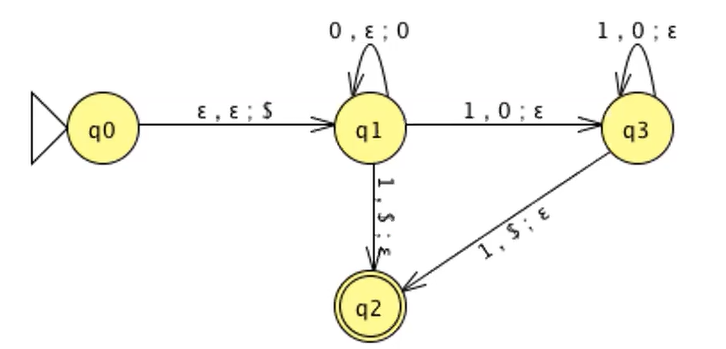
\includegraphics[scale=0.7]{../assets/pda_1.png}
        \end{center}
    \end{mdframed}

    \item Describe how your PDA works with the input \code{00111}.
    \begin{mdframed}[]
        \begin{itemize}
            \item For our initial step, we start at $q_0$ and our stack can be described as \code{[]}.
            \item Looking at the only transition arrow, note that we can transition without reading any input ($\epsilon, \epsilon \mapsto \$$). Upon transitioning, we don't pop anything from the stack, but we do push the special \code{\$} onto the stack. So, we can describe the machine like so: 
            \begin{verbatim}
                State:  q1
                Stack:  [$]     Top 
                Input:  00111
                        ^
            \end{verbatim}

            \item At $q_1$, we have three transition arrows; one that requires a \code{0} (without reading and popping anything from the stack), and two that requires a \code{1} (one which requires the \code{\$} to be at the top of the stack, and another that requires a \code{0} to be on top of the stack). As the (first and) next symbol in our input is \code{0}, we read that in and transition to $q_1$ again while also pushing \code{0} onto the stack. 
            \begin{verbatim}
                State:  q1
                Stack:  [$, 0]     Top 
                Input:  00111
                         ^         Next to read
            \end{verbatim}

            \item We repeat the previous step since we need to read in a \code{0}. 
            \begin{verbatim}
                State:  q1
                Stack:  [$, 0, 0]     Top 
                Input:  00111
                          ^           Next to read
            \end{verbatim}

            \item At this point, our next input symbol is \code{1}. As we're at $q_1$ still, we now need to consider the two transition arrows that can read in a \code{1}. One transition arrow requires a \code{0} to be on top of the stack, and another requires a \code{\$}. So, we go with the one that requires a \code{0} to be on top of the stack since that's what we have in the stack. So, we transition to $q_3$, popping a \code{0} from the stack. 
            \begin{verbatim}
                State:  q2
                Stack:  [$, 0]     Top 
                Input:  00111
                           ^       Next to read
            \end{verbatim}
            
            \item We are now at state $q_3$. The next input symbol we need to read in is the \code{1} (the center one), and we still have another \code{0} on top of the stack. So, we take the transition arrow $\code{1}, \code{0} \mapsto \epsilon$. After transitioning back to $q_3$, we pop \code{0} from the stack. 
            \begin{verbatim}
                State:  q2
                Stack:  [$]     Top 
                Input:  00111
                            ^   Next to read
            \end{verbatim}

            \item Now that we're still at $q_3$, we still need to read in \code{1} (the last one). However, the top of the stack is a \code{\$}, implying that we're at the end of the stack. We note that there is a transition arrow $\code{1}, \$ \mapsto \epsilon$, we take that transition arrow. So, we transition to $q_2$ and pop \code{\$} from the stack. 
            \begin{verbatim}
                State:  q2
                Stack:  []     Top 
                Input:  00111
                             ^ Next to read
            \end{verbatim}

            \item There is nothing left to read, and since we're at $q_2$, we accept.
        \end{itemize}

        For a summary of what just happened, observe the below table.
        \begin{center}
            \begin{tabular}{c|c|c}
                \textbf{Input} & $q$ & \textbf{Stack} (Top is Right) \\ 
                \hline 
                               & $q_0$ & \code{[]} \\ 
                               & $q_1$ & \code{[\$]} \\ 
                \code{0}       & $q_1$ & \code{[\$, 0]} \\ 
                \code{0}       & $q_1$ & \code{[\$, 0, 0]} \\ 
                \code{1}       & $q_3$ & \code{[\$, 0]} \\ 
                \code{1}       & $q_3$ & \code{[\$]} \\ 
                \code{1}       & $q_2$ & \code{[]} \\ 
            \end{tabular}
        \end{center}
    \end{mdframed}
\end{enumerate}

\subsubsection{Example 2: PDA vs. CFGs}
Consider the following language $L = \{\code{a}^i \code{b}^j \code{c}^k \mid i = j \text{ or } i = k \text{ with } i, j, k \geq 0\}$. 

\begin{enumerate}
    \item Which of the following strings are \textbf{not} in $L$?
    \begin{itemize}
        \item \code{b}
        \item \code{abc}
        \item \code{abbcc}
        \item \code{aabcc}
    \end{itemize}

    \begin{mdframed}[]
        The answer is \code{abbcc}. This says that $i = 1$, $j = k = 2$, but this violates the definition that $i = j$ or $i = k$ since $i \neq j$ and $i \neq k$. 
    \end{mdframed}


    \item Create a CFG that generates $L$. 
    \begin{mdframed}[]
        The idea is that 
        \begin{equation*}
            \begin{aligned}
                L &= \{\code{a}^i \code{b}^j \code{c}^k \mid i = j \text{ or } i = k \text{ with } i, j, k \geq 0\} \\ 
                    &= \{\code{a}^i \code{b}^j \code{c}^k \mid i = j \text{ with } i, j, k \geq 0\} \cup \{\code{a}^i \code{b}^j \code{c}^k \mid i = k \text{ with } i, j, k \geq 0\}
            \end{aligned}
        \end{equation*}
        So, we can find the CFG of each individual language and then combine them to form the CFG of interest. 

        \begin{itemize}
            \item $L_1 = \{\code{a}^i \code{b}^j \code{c}^k \mid i = j \text{ with } i, j, k \geq 0\}$. The CFG can be defined by 
            \begin{equation*}
                \begin{aligned}
                    A &\mapsto A\code{c} \mid B \\ 
                    B &\mapsto \code{a}B\code{b} \mid \epsilon
                \end{aligned}
            \end{equation*}

            \item $L_2 = \{\code{a}^i \code{b}^j \code{c}^k \mid i = k \text{ with } i, j, k \geq 0\}$. The CFG can be defined by 
            \begin{equation*}
                \begin{aligned}
                    C &\mapsto \code{a}C\code{c} \mid D \\ 
                    D &\mapsto D\code{b} \mid \epsilon
                \end{aligned}
            \end{equation*}
        \end{itemize}

        Combining these gives us 
        \begin{equation*}
            \begin{aligned}
                S &\mapsto A \mid C \\ 
                A &\mapsto A\code{c} \mid B \\ 
                B &\mapsto \code{a}B\code{b} \mid \epsilon \\ 
                C &\mapsto \code{a}C\code{c} \mid D \\ 
                D &\mapsto D\code{b} \mid \epsilon
            \end{aligned}
        \end{equation*}
    \end{mdframed}

    \item Give an informal description of a PDA that accepts all strings in this language. \emph{Hint:} Consider what information you need to track, the amount of memory you need, and whether non-determinism is needed.
    
    \begin{mdframed}[]
        \begin{itemize}
            \item The PDA pushes a \code{\$} to indicate the top of the stack. Then, it starts reading \code{a}'s, pushing each one onto the top of the stack.
            \item The PDA then guesses when it has reached the end of the \code{a}'s and whether to match the number of \code{a}'s to the number of \code{b}'s or the number of \code{c}'s. 
            \item If trying to match number of \code{b}'s with the number of \code{a}'s, the PDA pops off \code{a}'s for each \code{b} that is read in. If there are more \code{a}'s on the stack but no more \code{b}'s being read, then we reject. When the end of the stack \code{\$} is reached, the number of \code{a}'s matches the number of \code{b}'s. If this is the end of the input or if any number of \code{c}'s is read at this point, accept. Otherwise, reject. 
            \item If trying to match the number of \code{c}'s with the number of \code{a}'s, first read any number of \code{b}'s without changing the stack content. Then, nondeterministically guess when to start reading the \code{c}'s. For each \code{c} read, pop one \code{a} off the stack. When the end of the stack \code{\$} is reached, the number of \code{a}'s and \code{c}'s match. 
        \end{itemize}
    \end{mdframed}

    \item Design a PDA that does exactly what you described in the previous step. 
    \begin{mdframed}[nobreak=true]
        \begin{center}
            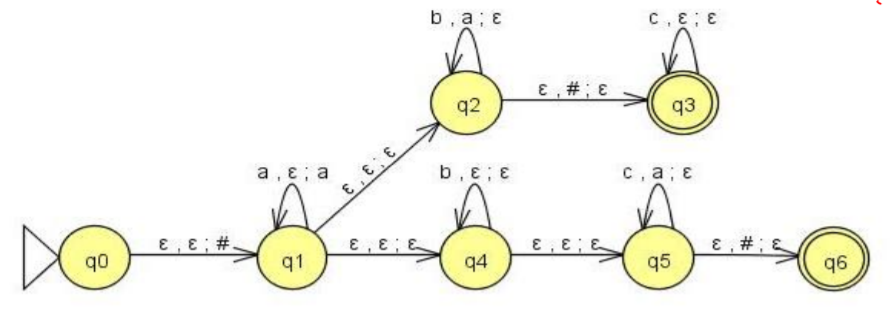
\includegraphics[scale=0.6]{../assets/pda_2.png}
        \end{center}
    \end{mdframed}
\end{enumerate}

\subsection{Conventions for PDAs}
\begin{itemize}
    \item We can \emph{test for the end of the stack}, without providing details. We can always push the end-of-stack symbol \code{\$} at the start. 
    \item We can \emph{test for the end of the input} without providing details. We can transform the PDA to one where accepting states are only those reachable when there are no more input symbols. 
    \item We don't always need to provide a state transition diagram.
\end{itemize}


\end{document}